\section{\ac{SAT}-солверы}

Сравнивать SMT с SAT, это как сравнивать высокоуровневый ЯП с языком ассемблера.
Последний может быть куда более эффективным, но на нем труднее программировать.

\subsection{CNF форма}

\ac{CNF}\footnote{\url{https://en.wikipedia.org/wiki/Conjunctive_normal_form}} это так называемая \textit{нормальная форма}.

% TODO recheck
% TODO write abt it!
%\textit{normal form} is somewhat similar to polynomials in algebra. 
%What is polynomial?
%It is a standard way to express unsystematic equations like $2x \cdot x$ as $3x$ polynomial, 
%and so you will be able to apply some operations to polynomials like summing, etc.

Любое булево выражение может быть сконвертировано в \textit{нормальную форму}, и \ac{CNF} это одна из них.
\ac{CNF}-выражение это пачка клозов (подвыражений) состоящих их литералов (или термов, переменных), операций ИЛИ и НЕ,
все из которых склеены друг с другом в полное выражение операцией И.
Вот способ запомнить: \ac{CNF} это ``И всех ИЛИ'' (или ``произведение всех сумм'')
и \ac{DNF} это ``ИЛИ всех И'' (или ``сумма всех произведений'').

Пример: $(\neg A \vee B) \wedge (C \vee \neg D)$.

$\vee$ означает ИЛИ (логическая дизьюнкция\footnote{\url{https://en.wikipedia.org/wiki/Logical_disjunction}}), 
знак ``+'' также иногда используется для ИЛИ.

$\wedge$ означает ИЛИ (логическая коньюнкция\footnote{\url{https://en.wikipedia.org/wiki/Logical_conjunction}}).
Легко запомнить: $\wedge$ выглядит как буква ``A''.
Знак ``$\cdot$'' также иногда используется для И.

$\neg$ это отрицание (НЕ).

% TODO A/B is the first clause, C/D is second

\subsection{Пример: двухбитный сумматор}
\label{adder}

В сущности, \ac{SAT}-солвер это солвер огромных булевых уравнений в CNF-форме.
Он просто выдает ответ, есть ли набор входных значений, удовлетворяющий CNF-выражению, и какие это значения должны быть.

Вот для примера двухбитный сумматор:

\begin{figure}[ht!]
\centering
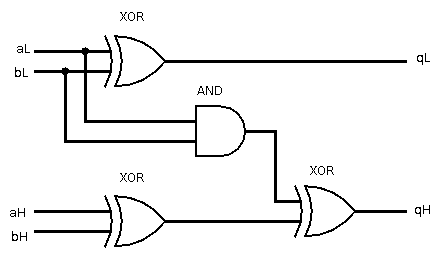
\includegraphics[scale=0.75]{SAT/adder_logisim.png}
\caption{Схема двухбитного сумматора}
\end{figure}

Сумматор здесь в самом простом возможном виде: у него нет входных и выходных переносов, и тут только 3 XOR-гейта
и один AND-гейт.
Попробуем разобраться, какой набор входных переменных заставит сумматор выставить оба выходных бита?
Просто подсчитав в уме, мы можем увидеть, что таких способа 4: $0+3=3$, $1+2=3$, $2+1=3$, $3+0=3$.
Вот также таблица истинности, с подсвеченными соответствующими рядами:

\newcommand{\HLcell}{\cellcolor{blue!25}}

\begin{center}
\begin{doublespace}
\noindent\(\begin{array}{l|llllll}
  & \text{aH} & \text{aL} & \text{bH} & \text{bL} & \text{qH} & \text{qL} \\
\hline
 \text{3+3 = 6 $\equiv $ 2 (mod 4)} & 1 & 1 & 1 & 1 & 1 & 0 \\
 \text{3+2 = 5 $\equiv $ 1 (mod 4)} & 1 & 1 & 1 & 0 & 0 & 1 \\
 \text{3+1 = 4 $\equiv $ 0 (mod 4)} & 1 & 1 & 0 & 1 & 0 & 0 \\
 \text{\HLcell{}3+0 = 3 $\equiv $ 3 (mod 4)} & \HLcell{}1 & \HLcell{}1 & \HLcell{}0 & \HLcell{}0 & \HLcell{}1 & \HLcell{}1 \\
 \text{2+3 = 5 $\equiv $ 1 (mod 4)} & 1 & 0 & 1 & 1 & 0 & 1 \\
 \text{2+2 = 4 $\equiv $ 0 (mod 4)} & 1 & 0 & 1 & 0 & 0 & 0 \\
 \text{\HLcell{}2+1 = 3 $\equiv $ 3 (mod 4)} & \HLcell{}1 & \HLcell{}0 & \HLcell{}0 & \HLcell{}1 & \HLcell{}1 & \HLcell{}1 \\
 \text{2+0 = 2 $\equiv $ 2 (mod 4)} & 1 & 0 & 0 & 0 & 1 & 0 \\
 \text{1+3 = 4 $\equiv $ 0 (mod 4)} & 0 & 1 & 1 & 1 & 0 & 0 \\
 \text{\HLcell{}1+2 = 3 $\equiv $ 3 (mod 4)} & \HLcell{}0 & \HLcell{}1 & \HLcell{}1 & \HLcell{}0 & \HLcell{}1 & \HLcell{}1 \\
 \text{1+1 = 2 $\equiv $ 2 (mod 4)} & 0 & 1 & 0 & 1 & 1 & 0 \\
 \text{1+0 = 1 $\equiv $ 1 (mod 4)} & 0 & 1 & 0 & 0 & 0 & 1 \\
 \text{\HLcell{}0+3 = 3 $\equiv $ 3 (mod 4)} & \HLcell{}0 & \HLcell{}0 & \HLcell{}1 & \HLcell{}1 & \HLcell{}1 & \HLcell{}1 \\
 \text{0+2 = 2 $\equiv $ 2 (mod 4)} & 0 & 0 & 1 & 0 & 1 & 0 \\
 \text{0+1 = 1 $\equiv $ 1 (mod 4)} & 0 & 0 & 0 & 1 & 0 & 1 \\
 \text{0+0 = 0 $\equiv $ 0 (mod 4)} & 0 & 0 & 0 & 0 & 0 & 0 \\
\end{array}\)
\end{doublespace}
\end{center}


Посмотрим, что об этом скажет SAT-солвер?

В начале, нам нужно представить наш двухбитный сумматор как CNF-выражение.

Используя Wolfram Mathematica, можно выразить 1-битное выражение для обоих выходов сумматоров:\\
\\
\textbf{\texttt{In[]:=AdderQ0[aL$\_$,bL$\_$]=Xor[aL,bL]}} \\
\textbf{\texttt{Out[]:=aL $\veebar$ bL}} \\
\\
\textbf{\texttt{In[]:=AdderQ1[aL$\_$,aH$\_$,bL$\_$,bH$\_$]=Xor[And[aL,bL],Xor[aH,bH]]}} \\
\textbf{\texttt{Out[]:=aH $\veebar$ bH $\veebar$ (aL \&\& bL)}} \\
\\
Нам нужно такое выражение, где обе части выдадут единицы.
Используя Wolfram Mathematica, найдем все возможные входы такого выражения (я склеил обе части при помощи And): \\
\\
\textbf{\texttt{In[]:=Boole[SatisfiabilityInstances[And[AdderQ0[aL,bL],AdderQ1[aL,aH,bL,bH]],\{aL,aH,bL,bH\},4]]}} \\
\textbf{\texttt{Out[]:=\{1,1,0,0\},\{1,0,0,1\},\{0,1,1,0\},\{0,0,1,1\}}} \\
\\
Да, действительно, Mathematica говорит, что здесь 4 входа, которые приведут к нужному нам результату.
Так что, Mathematica тоже может использоваться как \ac{SAT}-солвер.

Тем не менее, перейдем к CNF-форме. Используя Mathematica, сконвертируем наше выражение в CNF-форму:\\
\\
\textbf{\texttt{In[]:=cnf=BooleanConvert[And[AdderQ0[aL,bL],AdderQ1[aL,aH,bL,bH]],``CNF'']}} \\
\textbf{\texttt{Out[]:=(!aH $\|$ !bH) \&\& (aH $\|$ bH) \&\& (!aL $\|$ !bL) \&\& (aL $\|$ bL)}} \\
\\
Выглядит посложнее. Причина такой многословности в том, что \ac{CNF}-форма не поддерживает операцию исключающего
ИЛИ.
% FIXME: TeX form of the expression!

\subsubsection{MiniSat}

Для начала, попробуем MiniSat\footnote{\url{http://minisat.se/MiniSat.html}}.
Стандартный способ закодировать \ac{CNF}-выражение для MiniSat это перечислить все части ИЛИ в каждой строке.
Также, MiniSat не поддерживает имена переменных, только числа.
Перечислим наши переменные: 1 будет aH, 2 -- aL, 3 -- bH, 4 -- bL.

Вот что получилось, когда я сконвертировал выражение из Mathematica во входной файл для MiniSat:

\begin{lstlisting}
p cnf 4 4
-1 -3 0
1 3 0
-2 -4 0
2 4 0
\end{lstlisting}

Две четверки в первой строке это, соответственно, число переменных и число клозов.
Так что тут 4 строки, каждая для каждого клоза ИЛИ.
Минус перед номером переменной означает что переменная инвертирована.
Отсутствие минуса -- не инвертирована.
Ноль в конце это просто оконечивающий ноль, означающий конец клоза.

Другими словами, каждая строка это ИЛИ-клоз с возможными инвертированиями,
и задача MiniSat в том, чтобы найти такой набор входных переменных, который удовлетворит все строки во входном файле.

Этот файл я назвал \textit{adder.cnf} и теперь попробуем MiniSat:

\begin{lstlisting}
% minisat -verb=0 adder.cnf results.txt
SATISFIABLE
\end{lstlisting}

Результаты в файле \textit{results.txt}:

\begin{lstlisting}
SAT
-1 -2 3 4 0
\end{lstlisting}

Это означает, что если первые две переменных (aH и aL) будут \textit{false},
и две последние переменные (bH и bL) будут \textit{true},
все \ac{CNF}-выражение будет истинно (satisfiable).
Похоже на правду: если bH и bL выставить в \textit{true}, оба бита результата также будут \textit{true}.

Как получить другие решения (instances)?
\ac{SAT}-солверы, как и \ac{SMT}-солверы, выдают только одно решение (или \textit{instance}).

MiniSat использует \ac{PRNG}, и его изначальное состояние (seed) можно задать явно.
Я попробовал разные значения, но результат всё тот же.
Тем не менее, CryptoMiniSat в этом случае может показать все возможные 4 решения, хотя и в хаотичном порядке.
Так что это не очень надежный способ.

Видимо, единственный способ, это инвертировать клоз решения и добавить его во входное выражение.
Мы получили \TT{-1 -2 3 4}, 
теперь мы можем инвертировать все значения в нем (просто поменяйте минусы: \TT{1 2 -3 -4}),
и добавим это в конец входного файла:

\begin{lstlisting}
p cnf 4 5
-1 -3 0
1 3 0
-2 -4 0
2 4 0
1 2 -3 -4
\end{lstlisting}

Получаем другой результат:

\begin{lstlisting}
SAT
1 2 -3 -4 0
\end{lstlisting}

Это означает что обе aH и aL должны быть \textit{true} и bH и bL должны быть \textit{false}, чтобы удовлетворить
входное выражение.
Снова инвертируем это решение и снова добавим:

\begin{lstlisting}
p cnf 4 6
-1 -3 0
1 3 0
-2 -4 0
2 4 0
1 2 -3 -4
-1 -2 3 4 0
\end{lstlisting}

Результат:

\begin{lstlisting}
SAT
-1 2 3 -4 0
\end{lstlisting}

aH=false, aL=true, bH=true, bL=false. Это также корректно, в соответствии с таблицей истинности.

Добавим снова:

\begin{lstlisting}
p cnf 4 7
-1 -3 0
1 3 0
-2 -4 0
2 4 0
1 2 -3 -4
-1 -2 3 4 0
1 -2 -3 4 0
\end{lstlisting}

\begin{lstlisting}
SAT
1 -2 -3 4 0
\end{lstlisting}

\textit{aH=true, aL=false, bH=false, bL=true.} Это тоже верно.

Это четвертый результат. Больше быть не должно. Что если добавим и это?

\begin{lstlisting}
p cnf 4 8
-1 -3 0
1 3 0
-2 -4 0
2 4 0
1 2 -3 -4
-1 -2 3 4 0
1 -2 -3 4 0
-1 2 3 -4 0
\end{lstlisting}

Теперь MiniSat просто говорит ``UNSATISFIABLE'' без всякой дополнительной информации в файле результатов.

Нам пример крохотный, но MiniSat может работать с огромными \ac{CNF}-выражениями.

\subsubsection{CryptoMiniSat}

Операция исключающего ИЛИ (XOR) отсутствует в CNF-форме, но она очень важна в криптографических алгоритмах.
Простейший способ представить одну единственную XOR-операцию в CNF-форме, это:
$(\neg x \vee \neg y) \wedge (x \vee y)$ -- не очень короткое выражение,
хотя, множество XOR-операций в одном выражении могут оптимизироваться лучше.

Одна значительная разница между MiniSat и CryptoMiniSat в том, что последний поддерживает
клозы с операцией XOR вместо ИЛИ,
потому что CryptoMiniSat предназначен больше для анализа криптоалгоритмов\footnote{\url{http://www.msoos.org/xor-clauses/}}.
XOR-клозы поддерживаются в CryptoMiniSat специальным образом, без трансляции в клозы ИЛИ.

Вам нужно просто прибавить ``x'' к клозу в \ac{CNF}-файле и CryptoMiniSat затем считает обычный ИЛИ-клоз как XOR-клоз.
Что до двухбитного сумматора, вот самое короткое из возможных XOR-CNF выражений, которое можно использовать
для поиска всех входных значений, где оба выходных бита выставлены:

$(aH \oplus bH) \wedge (aL \oplus bL)$

Это \TT{.cnf}-файл CryptoMiniSat:

\begin{lstlisting}
p cnf 4 2
x1 3 0
x2 4 0
\end{lstlisting}

Запускаю CryptoMiniSat с разными значениями для инициализации его \ac{PRNG} \dots

\begin{lstlisting}
% cryptominisat4 --verb 0 --random 0 XOR_adder.cnf
s SATISFIABLE
v 1 2 -3 -4 0
% cryptominisat4 --verb 0 --random 1 XOR_adder.cnf
s SATISFIABLE
v -1 -2 3 4 0
% cryptominisat4 --verb 0 --random 2 XOR_adder.cnf
s SATISFIABLE
v 1 -2 -3 4 0
% cryptominisat4 --verb 0 --random 3 XOR_adder.cnf
s SATISFIABLE
v 1 2 -3 -4 0
% cryptominisat4 --verb 0 --random 4 XOR_adder.cnf
s SATISFIABLE
v -1 2 3 -4 0
% cryptominisat4 --verb 0 --random 5 XOR_adder.cnf
s SATISFIABLE
v -1 2 3 -4 0
% cryptominisat4 --verb 0 --random 6 XOR_adder.cnf
s SATISFIABLE
v -1 -2 3 4 0
% cryptominisat4 --verb 0 --random 7 XOR_adder.cnf
s SATISFIABLE
v 1 -2 -3 4 0
% cryptominisat4 --verb 0 --random 8 XOR_adder.cnf
s SATISFIABLE
v 1 2 -3 -4 0
% cryptominisat4 --verb 0 --random 9 XOR_adder.cnf
s SATISFIABLE
v 1 2 -3 -4 0
\end{lstlisting}

Тем не менее, все 4 возможных решения, это:

\begin{lstlisting}
v -1 -2 3 4 0
v -1 2 3 -4 0
v 1 -2 -3 4 0
v 1 2 -3 -4 0
\end{lstlisting}

\dots то же, что и выдал MiniSat.

% subsections:
\subsection{Взлом Сапёра при помощи SAT}
\label{minesweeper_SAT}

См.также о взломе оного при помощи Z3: \ref{minesweeper_SMT}.

\subsubsection{Простая ф-ция подсчета бит (\textit{population count})}

Прежде всего, нам нужно как считать количество соседних бомб.
Ф-ция подсчета та же, что и ф-ция подсчета бит (\textit{population count}).

Мы можем создать \ac{CNF}-выражение используя Wolfram Mathematica.
Это будет ф-ция, возвращающая \textit{True} если любые из двух бит 8-битного входа равняются \textit{True},
а остальные --- \textit{False}.
В начале, сделаем таблицу истинности для такой ф-ции:

\begin{lstlisting}
In[]:= tbl2 = 
 Table[PadLeft[IntegerDigits[i, 2], 8] -> 
   If[Equal[DigitCount[i, 2][[1]], 2], 1, 0], {i, 0, 255}]

Out[]= {{0, 0, 0, 0, 0, 0, 0, 0} -> 0, {0, 0, 0, 0, 0, 0, 0, 1} -> 0, 
{0, 0, 0, 0, 0, 0, 1, 0} -> 0, {0, 0, 0, 0, 0, 0, 1, 1} -> 1, 
{0, 0, 0, 0, 0, 1, 0, 0} -> 0, {0, 0, 0, 0, 0, 1, 0, 1} -> 1, 
{0, 0, 0, 0, 0, 1, 1, 0} -> 1, {0, 0, 0, 0, 0, 1, 1, 1} -> 0, 
{0, 0, 0, 0, 1, 0, 0, 0} -> 0, {0, 0, 0, 0, 1, 0, 0, 1} -> 1, 
{0, 0, 0, 0, 1, 0, 1, 0} -> 1, {0, 0, 0, 0, 1, 0, 1, 1} -> 0, 
...
{1, 1, 1, 1, 1, 0, 1, 0} -> 0, {1, 1, 1, 1, 1, 0, 1, 1} -> 0, 
{1, 1, 1, 1, 1, 1, 0, 0} -> 0, {1, 1, 1, 1, 1, 1, 0, 1} -> 0, 
{1, 1, 1, 1, 1, 1, 1, 0} -> 0, {1, 1, 1, 1, 1, 1, 1, 1} -> 0}
\end{lstlisting}

Теперь можем сделать \ac{CNF}-выражение используя эту таблицу истинности:

\begin{lstlisting}
In[]:= BooleanConvert[
 BooleanFunction[tbl2, {a, b, c, d, e, f, g, h}], "CNF"]

Out[]= (! a || ! b || ! c) && (! a || ! b || ! d) && (! a || ! 
    b || ! e) && (! a || ! b || ! f) && (! a || ! b || ! g) && (! 
    a || ! b || ! h) && (! a || ! c || ! d) && (! a || ! c || ! 
    e) && (! a || ! c || ! f) && (! a || ! c || ! g) && (! a || ! 
    c || ! h) && (! a || ! d || ! e) && (! a || ! d || ! f) && (! 
    a || ! d || ! g) && (! a || ! d || ! h) && (! a || ! e || ! 
    f) && (! a || ! e || ! g) && (! a || ! e || ! h) && (! a || ! 
    f || ! g) && (! a || ! f || ! h) && (! a || ! g || ! h) && (a || 
   b || c || d || e || f || g) && (a || b || c || d || e || f || 
   h) && (a || b || c || d || e || g || h) && (a || b || c || d || f ||
    g || h) && (a || b || c || e || f || g || h) && (a || b || d || 
   e || f || g || h) && (a || c || d || e || f || g || 
   h) && (! b || ! c || ! d) && (! b || ! c || ! e) && (! b || ! 
    c || ! f) && (! b || ! c || ! g) && (! b || ! c || ! h) && (! 
    b || ! d || ! e) && (! b || ! d || ! f) && (! b || ! d || ! 
    g) && (! b || ! d || ! h) && (! b || ! e || ! f) && (! b || ! 
    e || ! g) && (! b || ! e || ! h) && (! b || ! f || ! g) && (! 
    b || ! f || ! h) && (! b || ! g || ! h) && (b || c || d || e || 
   f || g || 
   h) && (! c || ! d || ! e) && (! c || ! d || ! f) && (! c || ! 
    d || ! g) && (! c || ! d || ! h) && (! c || ! e || ! f) && (! 
    c || ! e || ! g) && (! c || ! e || ! h) && (! c || ! f || ! 
    g) && (! c || ! f || ! h) && (! c || ! g || ! h) && (! d || ! 
    e || ! f) && (! d || ! e || ! g) && (! d || ! e || ! h) && (! 
    d || ! f || ! g) && (! d || ! f || ! h) && (! d || ! g || ! 
    h) && (! e || ! f || ! g) && (! e || ! f || ! h) && (! e || ! 
    g || ! h) && (! f || ! g || ! h)
\end{lstlisting}

Синтаксис такой же как и в Си/Си++
Проверим.

Я написал Питоновскую ф-цию для конвертирования вывода Mathematica в \ac{CNF}-файл, который можно подать на вход
SAT-солверу:

\lstinputlisting{SAT/minesweeper/tst.py}

Она заменяет переменные a/b/c/... на переданные имена переменных (1/2/3...), перерабатыает синтаксис, итд.
Вот результат:

\lstinputlisting{SAT/minesweeper/tst1.cnf}

Могу запустить:

\begin{lstlisting}
% minisat -verb=0 tst1.cnf results.txt
SATISFIABLE

% cat results.txt
SAT
1 -2 -3 -4 -5 -6 -7 8 0
\end{lstlisting}

Имя переменной в результате без знака минуса, это \textit{True}.
Имя переменной со знаком минус, это \textit{False}.
Мы здесь видим только две переменных \textit{True}: 1 и 8.
Это действительно корректно: солвер MiniSat нашел условие, для которого наша ф-ция возвращает \textit{True}.
Ноль в конце это просто терминирующий символ, который ничего не означает.

Мы можем попросить MiniSat найти еще одно решение, добавив текущее решение во входной CNF-файл,
но где все переменные инвертированы:

\begin{lstlisting}
...
-5 -6 -8 0
-5 -7 -8 0
-6 -7 -8 0
-1 2 3 4 5 6 7 -8 0
\end{lstlisting}

В обычном русском языке, это означает ``дайте ЛЮБОЕ решение, которые удовлетворяет все клозы, но также не равно
последнему клозу, которое мы только что добавили''.

MiniSat, действительно, находит еще одно решение, и снова, только с двумя переменными, равными \textit{True}:

\begin{lstlisting}
% minisat -verb=0 tst2.cnf results.txt
SATISFIABLE

% cat results.txt
SAT
1 2 -3 -4 -5 -6 -7 -8 0
\end{lstlisting}

Кстати, ф-ция \textit{population count} для 8-и соседей (POPCNT8) в CNF-форме, самая простая:

\begin{lstlisting}
a&&b&&c&&d&&e&&f&&g&&h
\end{lstlisting}

Действительно: она истинна, если все 8 входных бит тоже истинны.

Ф-ция для отсутствия соседей (POPCNT0) тоже очень простая:

\begin{lstlisting}
!a&&!b&&!c&&!d&&!e&&!f&&!g&&!h
\end{lstlisting}

Это означает, что она вернет \textit{True}, если все входные переменные \textit{False}.

Кстати, ф-ция POPCNT1 тоже простая:

\begin{lstlisting}
(!a||!b)&&(!a||!c)&&(!a||!d)&&(!a||!e)&&(!a||!f)&&(!a||!g)&&(!a||!h)&&(a||b||c||d||e||f||g||h)&&
(!b||!c)&&(!b||!d)&&(!b||!e)&&(!b||!f)&&(!b||!g)&&(!b||!h)&&(!c||!d)&&(!c||!e)&&(!c||!f)&&(!c||!g)&&
(!c||!h)&&(!d||!e)&&(!d||!f)&&(!d||!g)&&(!d||!h)&&(!e||!f)&&(!e||!g)&&(!e||!h)&&(!f||!g)&&(!f||!h)&&(!g||!h)
\end{lstlisting}

Здесь просто перечисление всех возможных пар 8-и переменных
(a/b, a/c, a/d, итд), что подразумевает: не должно присутствовать одновременно двух бит в каждой возможной паре.
И еще один клоз: ``(a||b||c||d||e||f||g||h)'', что подразумевает: минимум один бит должен присутствовать
среди 8-и переменных.

И да, вы можете использовать Mathematica для поиска \ac{CNF}-выражения для любой другой таблицы истинности.

\subsubsection{Сапёр}

Теперь можем использовать Mathematica для генерации всех ф-ций \textit{population count} для количества соседей 0..8.

Для Сапёра с матрицей $9 \cdot 9$ включая невидимую рамку, здесь будет $11 \cdot 11=121$ переменных,
связанных с матрицей Сапёра вот так:

\begin{lstlisting}
 1    2   3   4   5   6   7   8   9  10  11
12   13  14  15  16  17  18  19  20  21  22
23   24  25  26  27  28  29  30  31  32  33
34   35  36  37  38  39  40  41  42  43  44

...

100 101 102 103 104 105 106 107 108 109 110
111 112 113 114 115 116 117 118 119 120 121
\end{lstlisting}

Потом мы пишем Питоновский скрипт, складывающий все ф-ции \textit{population count}:
каждая ф-ция для каждого известного числа соседей (число на поле Сапёра).
Каждая ф-ция POPCNTx() берет на вход список переменных и выдает список клозов, которые будут добавлены
в итоговый \ac{CNF}-файл.

Что до пустых клеток, мы тоже добавляем их как клозы, но со знаком минус, что означает, что переменная
должна быть \textit{False}.
А когда мы пытаемся поместить бомбу, мы добавляем её переменную как клоз без знака минуса, что означает
что переменная должна быть \textit{True}.

Затем запускаем внешний процесс minisat.
Всё что нам от него нужно, это код возврата.
Если входной \ac{CNF} это \TT{UNSAT}, он возвращает 20:

Мы также используем здесь информацию из предыдущего решения Сапёра: \ref{minesweeper_SMT}.

\lstinputlisting{SAT/minesweeper/minesweeper_SAT.py}

( \url{https://github.com/dennis714/SAT_SMT_article/blob/master/SAT/minesweeper/minesweeper_SAT.py} ) \\
\\
Выходной \ac{CNF}-файл большой, вплоть до $\approx 2000$ клозов, и даже больше, вот, например: \url{https://github.com/dennis714/SAT_SMT_article/blob/master/SAT/minesweeper/sample.cnf}.

Так или иначе, это работает так же, как мой предыдущий скрипт для Z3Py:

\begin{lstlisting}
row=1, col=3, unsat!
row=6, col=2, unsat!
row=6, col=3, unsat!
row=7, col=4, unsat!
row=7, col=9, unsat!
row=8, col=9, unsat!
\end{lstlisting}

\dots но работает намного быстрее, даже учитывая запуск внешней программы.
Вероятно, версию для Z3Py можно было бы оптимизировать получше?

Файлы, включая файл для Wolfram Mathematica: \url{https://github.com/dennis714/SAT_SMT_article/tree/master/SAT/minesweeper}.


\subsection{Игра ``Жизнь'' Конвея}

\subsubsection{Откатывание состояния игры ``Жизнь'' назад}

Можно ли откатить назад известное состояние игры?
Это можно решить брутфорсом, но это экстремально медленно и неэффективно.

Попробуем SAT-солвер.

В начале, нужно определить ф-цию, которая будет говорить, будет ли новая клетка создаваться/рождаться, сохраняться/оставаться
или умирать.
Краткое напоминание: клетка рождается, если у нее 3 соседа, она остается живой, если у нее 2 или 3 соседа, она умирает
в остальных случаях.

Вот как я могу определить ф-цию, отражающую состояние новой клетки для следующего состояния:

\begin{lstlisting}
if center==true:
	return popcnt2(neighbours) || popcnt3(neighbours)
if center==false
	return popcnt3(neighbours)
\end{lstlisting}

Мы можем избавиться от конструкции ``if'':

\begin{lstlisting}
result=(center=true && (popcnt2(neighbours) || popcnt3(neighbours))) || (center=false && popcnt3(neighbours))
\end{lstlisting}

\dots где ``center'' это состояние центральной клетки, ``neighbours'' это 8 соседних клеток, popcnt2 это ф-ция,
возвращающая True если имеет на входе именно 2 бита, popcnt3 это тоже самое, только для 3-х бит
(такие же, как я использовал с своем примере с ``Сапёром'' (\ref{minesweeper_SAT})).

Используя Wolfram Mathematica, я в начале создаю функции-помошники и таблицу истинности для ф-ции, которая будет возвращать
\textit{true}, если ячейка должна присутствовать в следующем состоянии, либо \textit{false}, если нет:

\begin{lstlisting}
In[1]:= popcount[n_Integer]:=IntegerDigits[n,2] // Total

In[2]:= popcount2[n_Integer]:=Equal[popcount[n],2]

In[3]:= popcount3[n_Integer]:=Equal[popcount[n],3]

In[4]:= newcell[center_Integer,neighbours_Integer]:=(center==1 && (popcount2[neighbours]|| popcount3[neighbours]))||
(center==0 && popcount3[neighbours])

In[13]:= NewCellIsTrue=Flatten[Table[Join[{center},PadLeft[IntegerDigits[neighbours,2],8]] ->
Boole[newcell[center, neighbours]],{neighbours,0,255},{center,0,1}]]

Out[13]= {{0,0,0,0,0,0,0,0,0}->0,
{1,0,0,0,0,0,0,0,0}->0,
{0,0,0,0,0,0,0,0,1}->0,
{1,0,0,0,0,0,0,0,1}->0,
{0,0,0,0,0,0,0,1,0}->0,
{1,0,0,0,0,0,0,1,0}->0,
{0,0,0,0,0,0,0,1,1}->0,
{1,0,0,0,0,0,0,1,1}->1,

...

\end{lstlisting}

Теперь создаем \ac{CNF}-выражение из таблицы истинности:

\begin{lstlisting}
In[14]:= BooleanConvert[BooleanFunction[NewCellIsTrue,{center,a,b,c,d,e,f,g,h}],"CNF"]
Out[14]= (!a||!b||!c||!d)&&(!a||!b||!c||!e)&&(!a||!b||!c||!f)&&(!a||!b||!c||!g)&&(!a||!b||!c||!h)&&
(!a||!b||!d||!e)&&(!a||!b||!d||!f)&&(!a||!b||!d||!g)&&(!a||!b||!d||!h)&&(!a||!b||!e||!f)&&
(!a||!b||!e||!g)&&(!a||!b||!e||!h)&&(!a||!b||!f||!g)&&(!a||!b||!f||!h)&&(!a||!b||!g||!h)&&
(!a||!c||!d||!e)&&(!a||!c||!d||!f)&&(!a||!c||!d||!g)&&(!a||!c||!d||!h)&&(!a||!c||!e||!f)&&
(!a||!c||!e||!g)&&(!a||!c||!e||!h)&&(!a||!c||!f||!g)&&(!a||!c||!f||!h)&&

...

\end{lstlisting}

Также, нам нужна вторая ф-ция, \textit{инвертированная}, которая вернет \textit{true},
если ячейка должна отсутствовать в следующем состоянии, или \textit{false} в противном случае:

\begin{lstlisting}
In[15]:= NewCellIsFalse=Flatten[Table[Join[{center},PadLeft[IntegerDigits[neighbours,2],8]] ->
Boole[Not[newcell[center, neighbours]]],{neighbours,0,255},{center,0,1}]]
Out[15]= {{0,0,0,0,0,0,0,0,0}->1,
{1,0,0,0,0,0,0,0,0}->1,
{0,0,0,0,0,0,0,0,1}->1,
{1,0,0,0,0,0,0,0,1}->1,
{0,0,0,0,0,0,0,1,0}->1,

...

In[16]:= BooleanConvert[BooleanFunction[NewCellIsFalse,{center,a,b,c,d,e,f,g,h}],"CNF"]
Out[16]= (!a||!b||!c||d||e||f||g||h)&&(!a||!b||c||!d||e||f||g||h)&&(!a||!b||c||d||!e||f||g||h)&&
(!a||!b||c||d||e||!f||g||h)&&(!a||!b||c||d||e||f||!g||h)&&(!a||!b||c||d||e||f||g||!h)&&
(!a||!b||!center||d||e||f||g||h)&&(!a||b||!c||!d||e||f||g||h)&&(!a||b||!c||d||!e||f||g||h)&&
(!a||b||!c||d||e||!f||g||h)&&(!a||b||!c||d||e||f||!g||h)&&(!a||b||!c||d||e||f||g||!h)&&
(!a||b||c||!d||!e||f||g||h)&&(!a||b||c||!d||e||!f||g||h)&&(!a||b||c||!d||e||f||!g||h)&&

...

\end{lstlisting}

Используя тот же способ, что и в примере с ``Сапёром'', я могу конвертировать \ac{CNF}-выражение в список клозов:

\begin{lstlisting}
def mathematica_to_CNF (s, center, a):
    s=s.replace("center", center)
    s=s.replace("a", a[0]).replace("b", a[1]).replace("c", a[2]).replace("d", a[3])
    s=s.replace("e", a[4]).replace("f", a[5]).replace("g", a[6]).replace("h", a[7])
    s=s.replace("!", "-").replace("||", " ").replace("(", "").replace(")", "")
    s=s.split ("&&")
    return s
\end{lstlisting}

И снова, как в примере с ``Сапёром'', здесь есть невидимая рамка, чтобы сделать обработку проще.
Переменные в \ac{SAT} нумеруются как и в предыдущем примере:

\begin{lstlisting}
 1    2   3   4   5   6   7   8   9  10  11
12   13  14  15  16  17  18  19  20  21  22
23   24  25  26  27  28  29  30  31  32  33
34   35  36  37  38  39  40  41  42  43  44

...

100 101 102 103 104 105 106 107 108 109 110
111 112 113 114 115 116 117 118 119 120 121
\end{lstlisting}

Также, для упрощения, здесь есть и видимая рамка, всегда равняющаяся \textit{False}.

Теперь работающий исходник.
Всякий раз, когда встречаем ``*'' в \TT{final\_state[]}, мы добавляем клозы сгенерированные ф-цией
\TT{cell\_is\_true()}, или \TT{cell\_is\_false()}, если наоборот.
Когда получаем решение, мы его инвертируем и добавляем в список клозов, так что когда minisat будет исполняться
в следующий раз, он пропустит решение, которое только что было выведено.

\begin{lstlisting}
...

def cell_is_false (center, a):
    s="(!a||!b||!c||d||e||f||g||h)&&(!a||!b||c||!d||e||f||g||h)&&(!a||!b||c||d||!e||f||g||h)&&" \
      "(!a||!b||c||d||e||!f||g||h)&&(!a||!b||c||d||e||f||!g||h)&&(!a||!b||c||d||e||f||g||!h)&&" \
      "(!a||!b||!center||d||e||f||g||h)&&(!a||b||!c||!d||e||f||g||h)&&(!a||b||!c||d||!e||f||g||h)&&" \
      "(!a||b||!c||d||e||!f||g||h)&&(!a||b||!c||d||e||f||!g||h)&&(!a||b||!c||d||e||f||g||!h)&&" \
      "(!a||b||c||!d||!e||f||g||h)&&(!a||b||c||!d||e||!f||g||h)&&(!a||b||c||!d||e||f||!g||h)&&" \
      "(!a||b||c||!d||e||f||g||!h)&&(!a||b||c||d||!e||!f||g||h)&&(!a||b||c||d||!e||f||!g||h)&&" \
      "(!a||b||c||d||!e||f||g||!h)&&(!a||b||c||d||e||!f||!g||h)&&(!a||b||c||d||e||!f||g||!h)&&" \
      "(!a||b||c||d||e||f||!g||!h)&&(!a||!c||!center||d||e||f||g||h)&&(!a||c||!center||!d||e||f||g||h)&&" \
      "(!a||c||!center||d||!e||f||g||h)&&(!a||c||!center||d||e||!f||g||h)&&(!a||c||!center||d||e||f||!g||h)&&" \
      "(!a||c||!center||d||e||f||g||!h)&&(a||!b||!c||!d||e||f||g||h)&&(a||!b||!c||d||!e||f||g||h)&&" \
      "(a||!b||!c||d||e||!f||g||h)&&(a||!b||!c||d||e||f||!g||h)&&(a||!b||!c||d||e||f||g||!h)&&" \
      "(a||!b||c||!d||!e||f||g||h)&&(a||!b||c||!d||e||!f||g||h)&&(a||!b||c||!d||e||f||!g||h)&&" \
      "(a||!b||c||!d||e||f||g||!h)&&(a||!b||c||d||!e||!f||g||h)&&(a||!b||c||d||!e||f||!g||h)&&" \
      "(a||!b||c||d||!e||f||g||!h)&&(a||!b||c||d||e||!f||!g||h)&&(a||!b||c||d||e||!f||g||!h)&&" \
      "(a||!b||c||d||e||f||!g||!h)&&(a||b||!c||!d||!e||f||g||h)&&(a||b||!c||!d||e||!f||g||h)&&" \
      "(a||b||!c||!d||e||f||!g||h)&&(a||b||!c||!d||e||f||g||!h)&&(a||b||!c||d||!e||!f||g||h)&&" \
      "(a||b||!c||d||!e||f||!g||h)&&(a||b||!c||d||!e||f||g||!h)&&(a||b||!c||d||e||!f||!g||h)&&" \
      "(a||b||!c||d||e||!f||g||!h)&&(a||b||!c||d||e||f||!g||!h)&&(a||b||c||!d||!e||!f||g||h)&&" \
      "(a||b||c||!d||!e||f||!g||h)&&(a||b||c||!d||!e||f||g||!h)&&(a||b||c||!d||e||!f||!g||h)&&" \
      "(a||b||c||!d||e||!f||g||!h)&&(a||b||c||!d||e||f||!g||!h)&&(a||b||c||d||!e||!f||!g||h)&&" \
      "(a||b||c||d||!e||!f||g||!h)&&(a||b||c||d||!e||f||!g||!h)&&(a||b||c||d||e||!f||!g||!h)&&" \
      "(!b||!c||!center||d||e||f||g||h)&&(!b||c||!center||!d||e||f||g||h)&&(!b||c||!center||d||!e||f||g||h)&&" \
      "(!b||c||!center||d||e||!f||g||h)&&(!b||c||!center||d||e||f||!g||h)&&(!b||c||!center||d||e||f||g||!h)&&" \
      "(b||!c||!center||!d||e||f||g||h)&&(b||!c||!center||d||!e||f||g||h)&&(b||!c||!center||d||e||!f||g||h)&&" \
      "(b||!c||!center||d||e||f||!g||h)&&(b||!c||!center||d||e||f||g||!h)&&(b||c||!center||!d||!e||f||g||h)&&" \
      "(b||c||!center||!d||e||!f||g||h)&&(b||c||!center||!d||e||f||!g||h)&&(b||c||!center||!d||e||f||g||!h)&&" \
      "(b||c||!center||d||!e||!f||g||h)&&(b||c||!center||d||!e||f||!g||h)&&(b||c||!center||d||!e||f||g||!h)&&" \
      "(b||c||!center||d||e||!f||!g||h)&&(b||c||!center||d||e||!f||g||!h)&&(b||c||!center||d||e||f||!g||!h)"

    return mathematica_to_CNF(s, center, a)

def cell_is_true (center, a):
    s="(!a||!b||!c||!d)&&(!a||!b||!c||!e)&&(!a||!b||!c||!f)&&(!a||!b||!c||!g)&&(!a||!b||!c||!h)&&" \
      "(!a||!b||!d||!e)&&(!a||!b||!d||!f)&&(!a||!b||!d||!g)&&(!a||!b||!d||!h)&&(!a||!b||!e||!f)&&" \
      "(!a||!b||!e||!g)&&(!a||!b||!e||!h)&&(!a||!b||!f||!g)&&(!a||!b||!f||!h)&&(!a||!b||!g||!h)&&" \
      "(!a||!c||!d||!e)&&(!a||!c||!d||!f)&&(!a||!c||!d||!g)&&(!a||!c||!d||!h)&&(!a||!c||!e||!f)&&" \
      "(!a||!c||!e||!g)&&(!a||!c||!e||!h)&&(!a||!c||!f||!g)&&(!a||!c||!f||!h)&&(!a||!c||!g||!h)&&" \
      "(!a||!d||!e||!f)&&(!a||!d||!e||!g)&&(!a||!d||!e||!h)&&(!a||!d||!f||!g)&&(!a||!d||!f||!h)&&" \
      "(!a||!d||!g||!h)&&(!a||!e||!f||!g)&&(!a||!e||!f||!h)&&(!a||!e||!g||!h)&&(!a||!f||!g||!h)&&" \
      "(a||b||c||center||d||e||f)&&(a||b||c||center||d||e||g)&&(a||b||c||center||d||e||h)&&" \
      "(a||b||c||center||d||f||g)&&(a||b||c||center||d||f||h)&&(a||b||c||center||d||g||h)&&" \
      "(a||b||c||center||e||f||g)&&(a||b||c||center||e||f||h)&&(a||b||c||center||e||g||h)&&" \
      "(a||b||c||center||f||g||h)&&(a||b||c||d||e||f||g)&&(a||b||c||d||e||f||h)&&(a||b||c||d||e||g||h)&&" \
      "(a||b||c||d||f||g||h)&&(a||b||c||e||f||g||h)&&(a||b||center||d||e||f||g)&&(a||b||center||d||e||f||h)&&" \
      "(a||b||center||d||e||g||h)&&(a||b||center||d||f||g||h)&&(a||b||center||e||f||g||h)&&" \
      "(a||b||d||e||f||g||h)&&(a||c||center||d||e||f||g)&&(a||c||center||d||e||f||h)&&" \
      "(a||c||center||d||e||g||h)&&(a||c||center||d||f||g||h)&&(a||c||center||e||f||g||h)&&" \
      "(a||c||d||e||f||g||h)&&(a||center||d||e||f||g||h)&&(!b||!c||!d||!e)&&(!b||!c||!d||!f)&&" \
      "(!b||!c||!d||!g)&&(!b||!c||!d||!h)&&(!b||!c||!e||!f)&&(!b||!c||!e||!g)&&(!b||!c||!e||!h)&&" \
      "(!b||!c||!f||!g)&&(!b||!c||!f||!h)&&(!b||!c||!g||!h)&&(!b||!d||!e||!f)&&(!b||!d||!e||!g)&&" \
      "(!b||!d||!e||!h)&&(!b||!d||!f||!g)&&(!b||!d||!f||!h)&&(!b||!d||!g||!h)&&(!b||!e||!f||!g)&&" \
      "(!b||!e||!f||!h)&&(!b||!e||!g||!h)&&(!b||!f||!g||!h)&&(b||c||center||d||e||f||g)&&" \
      "(b||c||center||d||e||f||h)&&(b||c||center||d||e||g||h)&&(b||c||center||d||f||g||h)&&" \
      "(b||c||center||e||f||g||h)&&(b||c||d||e||f||g||h)&&(b||center||d||e||f||g||h)&&" \
      "(!c||!d||!e||!f)&&(!c||!d||!e||!g)&&(!c||!d||!e||!h)&&(!c||!d||!f||!g)&&(!c||!d||!f||!h)&&" \
      "(!c||!d||!g||!h)&&(!c||!e||!f||!g)&&(!c||!e||!f||!h)&&(!c||!e||!g||!h)&&(!c||!f||!g||!h)&&" \
      "(c||center||d||e||f||g||h)&&(!d||!e||!f||!g)&&(!d||!e||!f||!h)&&(!d||!e||!g||!h)&&(!d||!f||!g||!h)&&" \
      "(!e||!f||!g||!h)"

    return mathematica_to_CNF(s, center, a)

...
\end{lstlisting}

( \url{https://github.com/dennis714/SAT_SMT_article/blob/master/SAT/GoL/GoL_SAT_utils.py} )

\lstinputlisting{SAT/GoL/reverse1.py}

( \url{https://github.com/dennis714/SAT_SMT_article/blob/master/SAT/GoL/reverse1.py} )

И вот результат:

\begin{lstlisting}
HEIGHT= 3 WIDTH= 3
2525 clauses
.*.
*.*
.*.
1.rle written

2526 clauses
.**
*..
*.*
2.rle written

2527 clauses
**.
..*
*.*
3.rle written

2528 clauses
*.*
*..
.**
4.rle written

2529 clauses
*.*
..*
**.
5.rle written

2530 clauses
*.*
.*.
*.*
6.rle written

2531 clauses
unsat!
\end{lstlisting}

Первый результат такой же, как и изначальное состояние.
Действительно: это ``натюрморт'', т.е., состояние которое никогда не меняется, и это корректное решение.
Последнее решение также корректно.

Теперь проблема: 2-е, 3-е, 4-е и 5-е решения эквивалентны друг другу, они просто или отражены или повернуты.
На самом деле, это зеркальная\footnote{\url{https://en.wikipedia.org/wiki/Reflection_symmetry}} и 
ротационная\footnote{\url{https://en.wikipedia.org/wiki/Rotational_symmetry}} симметрии.
Мы можем это легко решить: мы будем брать каждое решение, отражать его и крутить, и добавлять в инвертированном виде
в список клозов, так что minisat при следующем запуске их пропустит:

\begin{lstlisting}

...

while True:
    solution=try_again(clauses)
    clauses.append(negate_clause(grid_to_clause(solution, H, W)))
    clauses.append(negate_clause(grid_to_clause(reflect_vertically(solution), H, W)))
    clauses.append(negate_clause(grid_to_clause(reflect_horizontally(solution), H, W)))
    # is this square?
    if W==H:
        clauses.append(negate_clause(grid_to_clause(rotate_square_array(solution,1), H, W)))
        clauses.append(negate_clause(grid_to_clause(rotate_square_array(solution,2), H, W)))
        clauses.append(negate_clause(grid_to_clause(rotate_square_array(solution,3), H, W)))
    print ""

...

\end{lstlisting}

( \url{https://github.com/dennis714/SAT_SMT_article/blob/master/SAT/GoL/reverse2.py} )

Ф-ции \TT{reflect\_vertically()}, \TT{reflect\_horizontally} and \TT{rotate\_squarearray()} просто преобразуют массив.

Теперь у нас всего 3 решения:

\begin{lstlisting}
HEIGHT= 3 WIDTH= 3
2525 clauses
.*.
*.*
.*.
1.rle written

2531 clauses
.**
*..
*.*
2.rle written

2537 clauses
*.*
.*.
*.*
3.rle written

2543 clauses
unsat!
\end{lstlisting}

У этого только один предок:

\begin{lstlisting}
final_state=[
" * ",
" * ",
" * "]
_PRE_END

_PRE_BEGIN
HEIGHT= 3 WIDTH= 3
2503 clauses
...
***
...
1.rle written

2509 clauses
unsat!
\end{lstlisting}

Это осциллятор, конечно.

Как много состояний могут привести к такой картинке?

\begin{lstlisting}
final_state=[
"  *  ",
"     ",
" **  ",
"  *  ",
"  *  ",
" *** "]
\end{lstlisting}

28, вот некоторые:

\begin{lstlisting}
HEIGHT= 6 WIDTH= 5
5217 clauses
.*.*.
..*..
.**.*
..*..
..*.*
.**..
1.rle written

5220 clauses
.*.*.
..*..
.**.*
..*..
*.*.*
.**..
2.rle written

5223 clauses
..*.*
..**.
.**..
....*
*.*.*
.**..
3.rle written

5226 clauses
..*.*
..**.
.**..
*...*
..*.*
.**..
4.rle written

...

\end{lstlisting}

Теперь самая большая, ``space invader'':

\begin{lstlisting}
final_state=[
"             ",
"   *     *   ",
"    *   *    ",
"   *******   ",
"  ** *** **  ",
" *********** ",
" * ******* * ",
" * *     * * ",
"    ** **    ",
"             "]
\end{lstlisting}

\begin{lstlisting}
HEIGHT= 10 WIDTH= 13
16469 clauses
..*.*.**.....
.....*****...
....**..*....
......*...*..
..**...*.*...
.*..*.*.**..*
*....*....*.*
..*.*..*.....
..*.....*.*..
....**..*.*..
1.rle written

16472 clauses
*.*.*.**.....
.....*****...
....**..*....
......*...*..
..**...*.*...
.*..*.*.**..*
*....*....*.*
..*.*..*.....
..*.....*.*..
....**..*.*..
2.rle written

16475 clauses
..*.*.**.....
*....*****...
....**..*....
......*...*..
..**...*.*...
.*..*.*.**..*
*....*....*.*
..*.*..*.....
..*.....*.*..
....**..*.*..
3.rle written

...

\end{lstlisting}

Не знаю, сколько возможных состояний могут привести к ``space invader''-у, вероятно, очень много.
Пришлось остановить.
И во время исполнения, вывод решений постепенно замедляется, потому что количество клозов возрастает
(из-за добавления инвертированных решений).

Все решения также экспортируются в RLE-файлы, которые можно открывать при помощи
Golly\footnote{\url{http://golly.sourceforge.net/}}.

\subsubsection{Поиск ``натюрмортов''}

``Натюрморт'' в терминах игры это состояние, которое вообще не меняется.

В начале, используя предыдущие определения, мы определим таблицу истинности для ф-ции, которая будет возвращать \textit{true},
если центральная клетка следующего состояния такая же, как она и была в предыдущем состоянии, т.е., она не менялась.

\begin{lstlisting}
In[17]:= stillife=Flatten[Table[Join[{center},PadLeft[IntegerDigits[neighbours,2],8]]->
Boole[Boole[newcell[center,neighbours]]==center],{neighbours,0,255},{center,0,1}]]
Out[17]= {{0,0,0,0,0,0,0,0,0}->1,
{1,0,0,0,0,0,0,0,0}->0,
{0,0,0,0,0,0,0,0,1}->1,
{1,0,0,0,0,0,0,0,1}->0,

...

In[18]:= BooleanConvert[BooleanFunction[stillife,{center,a,b,c,d,e,f,g,h}],"CNF"]
Out[18]= (!a||!b||!c||!center||!d)&&(!a||!b||!c||!center||!e)&&(!a||!b||!c||!center||!f)&&
(!a||!b||!c||!center||!g)&&(!a||!b||!c||!center||!h)&&(!a||!b||!c||center||d||e||f||g||h)&&
(!a||!b||c||center||!d||e||f||g||h)&&(!a||!b||c||center||d||!e||f||g||h)&&(!a||!b||c||center||d||e||!f||g||h)&&
(!a||!b||c||center||d||e||f||!g||h)&&(!a||!b||c||center||d||e||f||g||!h)&&(!a||!b||!center||!d||!e)&&

...

\end{lstlisting}

\lstinputlisting{SAT/GoL/stillife1.py}

( \url{https://github.com/dennis714/SAT_SMT_article/blob/master/SAT/GoL/stillife1.py} )

Что получим для $2 \cdot 2$?

\begin{lstlisting}
1881 clauses
..
..
1.rle written

1887 clauses
**
**
2.rle written

1893 clauses
unsat!
\end{lstlisting}

Оба решения корректы: пустой квадрат трансформируется в пустой квадрат (клетки не будут рождены).
Квадрат $2 \cdot 2$ также известен как ''натюрморт''.

Что насчет квадрата $3 \cdot 3$?

\begin{lstlisting}
2887 clauses
...
...
...
1.rle written

2893 clauses
.**
.**
...
2.rle written

2899 clauses
.**
*.*
**.
3.rle written

2905 clauses
.*.
*.*
**.
4.rle written

2911 clauses
.*.
*.*
.*.
5.rle written

2917 clauses
unsat!
\end{lstlisting}

Вот проблема: мы видим знакомый квадрат $2 \cdot 2$, но он сдвинут.
Это корректное решение, но нам оно не интересно, потому что мы его уже видели.

Что мы можем, это добавить еще одно условие. Мы можем заставить minisat искать решения без пустых рядов и столбцов.
Это легко.
Вот переменные в SAT для квадрата $5 \cdot 5$:

\begin{lstlisting}
1   2  3  4  5
6   7  8  9 10
11 12 13 14 15
16 17 18 19 20
21 22 23 24 25
\end{lstlisting}

Каждый клоз это клоз ``ИЛИ'', так что, всё что нужно, это добавить 5 клозов:

\begin{lstlisting}
1 OR 2 OR 3 OR 4 OR 5
6 OR 7 OR 8 OR 9 OR 10

...

\end{lstlisting}

Жто значит, что каждый ряд должен где-то иметь минимум одно значение \textit{True}.
Мы можем это делать и для каждого столбца.

\begin{lstlisting}

...

    # each row must contain at least one cell!
    for r in range(H):
        clauses.append(" ".join([coords_to_var(r, c, H, W) for c in range(W)]))

    # each column must contain at least one cell!
    for c in range(W):
        clauses.append(" ".join([coords_to_var(r, c, H, W) for r in range(H)]))

...

\end{lstlisting}

( \url{https://github.com/dennis714/SAT_SMT_article/blob/master/SAT/GoL/stillife2.py} )

Теперь мы видим, что квадрат $3 \cdot 3$ имеет 3 возможных натюрморта:

\begin{lstlisting}
2893 clauses
.*.
*.*
**.
1.rle written

2899 clauses
.*.
*.*
.*.
2.rle written

2905 clauses
.**
*.*
**.
3.rle written

2911 clauses
unsat!
\end{lstlisting}

$4 \cdot 4$ имеет 7:

\begin{lstlisting}
4169 clauses
..**
...*
***.
*...
1.rle written

4175 clauses
..**
..*.
*.*.
**..
2.rle written

4181 clauses
..**
.*.*
*.*.
**..
3.rle written

4187 clauses
..*.
.*.*
*.*.
**..
4.rle written

4193 clauses
.**.
*..*
*.*.
.*..
5.rle written

4199 clauses
..*.
.*.*
*.*.
.*..
6.rle written

4205 clauses
.**.
*..*
*..*
.**.
7.rle written

4211 clauses
unsat!
\end{lstlisting}

Когда я пробую большие квадраты, например $20 \cdot 20$, происходит смешное.
Прежде всего, minisat находит решение, не очень красивое эстетически, но всё же корректное, как:

\begin{lstlisting}
61033 clauses
....**.**.**.**.**.*
**..*.**.**.**.**.**
*...................
.*..................
**..................
*...................
.*..................
**..................
*...................
.*..................
**..................
*...................
.*..................
**..................
*...................
.*..................
..*.................
...*................
***.................
*...................
1.rle written

...

\end{lstlisting}

Действительно: все ряды и столбцы имеют миниму одно значение \textit{True}.

Затем minisat начинает добавлять маленькие натюрморты в общую картину:

\begin{lstlisting}
61285 clauses
.**....**...**...**.
.**...*..*.*.*...*..
.......**...*......*
..................**
...**............*..
...*.*...........*..
....*.*........**...
**...*.*...**..*....
*.*...*....*....*...
.*..........****.*..
................*...
..*...**..******....
.*.*..*..*..........
*..*...*.*..****....
***.***..*.*....*...
....*..***.**..**...
**.*..*.............
.*.**.**..........**
*..*..*..*......*..*
**..**..**......**..
43.rle written
\end{lstlisting}

Другими словами, результат это квадрат, состоящий из меньших натюрмортов.
Он затем немного меняет эти части, двигает их вперед и назад.
Это жульничество?
Так или иначе, он делает это в соответствии с четкими правилами, которые мы определили.

Но мы хотим более \textit{плотную} картину. Мы можем добавить правило: во всех кусках по 5 клеток должна быть
минимум одна \textit{True}-клетка.
Чтобы добиться этого, мы просто делим весь квадрат на куски по 5 клеток и добавляем клоз для каждого:

\begin{lstlisting}

...

    # make result denser:
    lst=[]
    for r in range(H):
        for c in range(W):
            lst.append(coords_to_var(r, c, H, W))
    # divide them all by chunks and add to clauses:
    CHUNK_LEN=5
    for c in list_partition(lst,len(lst)/CHUNK_LEN):
        tmp=" ".join(c)
        clauses.append(tmp)

...

\end{lstlisting}

( \url{https://github.com/dennis714/SAT_SMT_article/blob/master/SAT/GoL/stillife.py} )

Это действительно поплотнее:

\begin{lstlisting}
61113 clauses
..**.**......*.*.*..
...*.*.....***.**.*.
...*..*...*.......*.
....*.*..*.*......**
...**.*.*..*...**.*.
..*...*.***.....*.*.
...*.*.*......*..*..
****.*..*....*.**...
*....**.*....*.*....
...**..*...**..*....
..*..*....*....*.**.
.*.*.**....****.*..*
..*.*....*.*..*..**.
....*.****..*..*.*..
....**....*.*.**..*.
*.**...****.*..*.**.
**...**.....**.*....
...**..*..**..*.**.*
***.*.*..*.*..*.*.**
*....*....*....*....
1.rle written

61119 clauses
..**.**......*.*.*..
...*.*.....***.**.*.
...*..*...*.......*.
....*.*..*.*......**
...**.*.*..*...**.*.
..*...*.***.....*.*.
...*.*.*......*..*..
****.*..*....*.**...
*....**.*....*.*....
...**..*...**..*....
..*..*....*....*.**.
.*.*.**....****.*..*
..*.*....*.*..*..**.
....*.****..*..*.*..
....**....*.*.**..*.
*.**...****.*..*.**.
**...**.....**.*....
...**..*.***..*.**.*
***.*..*.*..*.*.*.**
*.......*..**.**....
2.rle written

...

\end{lstlisting}

Попробуем еще плотнее, одна обязательная \textit{true}-клетка для каждого 4-клеточного куска:

\begin{lstlisting}
61133 clauses
.**.**...*....**..**
*.*.*...*.*..*..*..*
*....*...*.*..*.**..
.***.*.....*.**.*...
..*.*.....**...*..*.
*......**..*...*.**.
**.....*...*.**.*...
...**...*...**..*...
**.*..*.*......*...*
.*...**.**..***.****
.*....*.*..*..*.*...
**.***...*.**...*.**
.*.*..****.....*..*.
*....*.....**..**.*.
*.***.*..**.*.....**
.*...*..*......**...
...*.*.**......*.***
..**.*.....**......*
*..*.*.**..*.*..***.
**....*.*...*...*...
1.rle written

61139 clauses
.**.**...*....**..**
*.*.*...*.*..*..*..*
*....*...*.*..*.**..
.***.*.....*.**.*...
..*.*.....**...*..*.
*......**..*...*.**.
**.....*...*.**.*...
...**...*...**..*...
**.*..*.*......*...*
.*...**.**..***.****
.*....*.*..*..*.*...
**.***...*.**...*.**
.*.*..****.....*..*.
*....*.....**..**.*.
*.***.*..**.*.....**
.*...*..*......**..*
...*.*.**......*.**.
..**.*.....**....*..
*..*.*.**..*.*...*.*
**....*.*...*.....**
2.rle written

...

\end{lstlisting}

\dots и даже больше: одна клетка на каждый 3-клеточный кусок:

\begin{lstlisting}
61166 clauses
**.*..**...**.**....
*.**..*.*...*.*.*.**
....**..*...*...*.*.
.**..*.*.**.*.*.*.*.
..**.*.*...*.**.*.**
*...*.*.**.*....*.*.
**.*..*...*.*.***..*
.*.*.*.***..**...**.
.*.*.*.*..**...*.*..
**.**.*..*...**.*..*
..*...*.**.**.*.*.**
..*.**.*..*.*.*.*...
**.*.*...*..*.*.*...
.*.*...*.**..*..***.
.*..****.*....**...*
..*.*...*..*...*..*.
.**...*.*.**...*.*..
..*..**.*.*...**.**.
..*.*..*..*..*..*..*
.**.**....**..**..**
1.rle written

61172 clauses
**.*..**...**.**....
*.**..*.*...*.*.*.**
....**..*...*...*.*.
.**..*.*.**.*.*.*.*.
..**.*.*...*.**.*.**
*...*.*.**.*....*.*.
**.*..*...*.*.***..*
.*.*.*.***..**...**.
.*.*.*.*..**...*.*..
**.**.*..*...**.*..*
..*...*.**.**.*.*.**
..*.**.*..*.*.*.*...
**.*.*...*..*.*.*...
.*.*...*.**..*..***.
.*..****.*....**...*
..*.*...*..*...*..*.
.**..**.*.**...*.*..
*..*.*..*.*...**.**.
*..*.*.*..*..*..*..*
.**...*...**..**..**
2.rle written

...

\end{lstlisting}

Это самое плотное. К несчастью, невозможно создать натюрморт с одной обязательной 
\textit{true}-клеткой в каждом 2-клеточном куске.

\subsubsection{Исходный код}

Исходный код и файл для Wolfram Mathematica: \url{https://github.com/dennis714/SAT_SMT_article/tree/master/SAT/GoL}.



